\section{Postgres-XC}
\label{sec:postgres-xc}

Postgres-XC~-- система для создания мульти-мастер кластеров, работающих в синхронном режиме~-- все узлы всегда содержат актуальные данные. Postgres-XC поддерживает опции для увеличения масштабирования кластера как при преобладании операций записи, так и при основной нагрузке на чтение данных: поддерживается выполнение транзакций с распараллеливанием на несколько узлов, за целостностью транзакций в пределах всего кластера отвечает специальный узел GTM (Global Transaction Manager).

Измерение производительности показало, что КПД кластера Postgres-XC составляет примерно 64\%, т.е. кластер из 10 серверов позволяет добиться увеличения производильности системы в целом в 6.4 раза, относительно производительности одного сервера (цифры приблизительные). 

Система не использует в своей работе триггеры и представляет собой набор дополнений и патчей к PostgreSQL, дающих возможность в прозрачном режиме обеспечить работу в кластере стандартных приложений, без их дополнительной модификации и адаптации (полная совместимость с PostgreSQL API). Кластер состоит из одного управляющего узла (GTM), предоставляющего информацию о состоянии транзакций, и произвольного набора рабочих узлов, каждый из которых в свою очередь состоит из координатора и обработчика данных (обычно эти элементы реализуются на одном сервере, но могут быть и разделены).

Хоть Postgres-XC и выглядит похожим на MultiMaster, но он им не является. Все сервера кластера должны быть соединены сетью с минимальными задержками, никакое географически-распределенное решение с разумной производительностью построить на нем не возможно (это важный момент).

\subsection{Архитектера}

\begin{figure}[ht!]
  \center{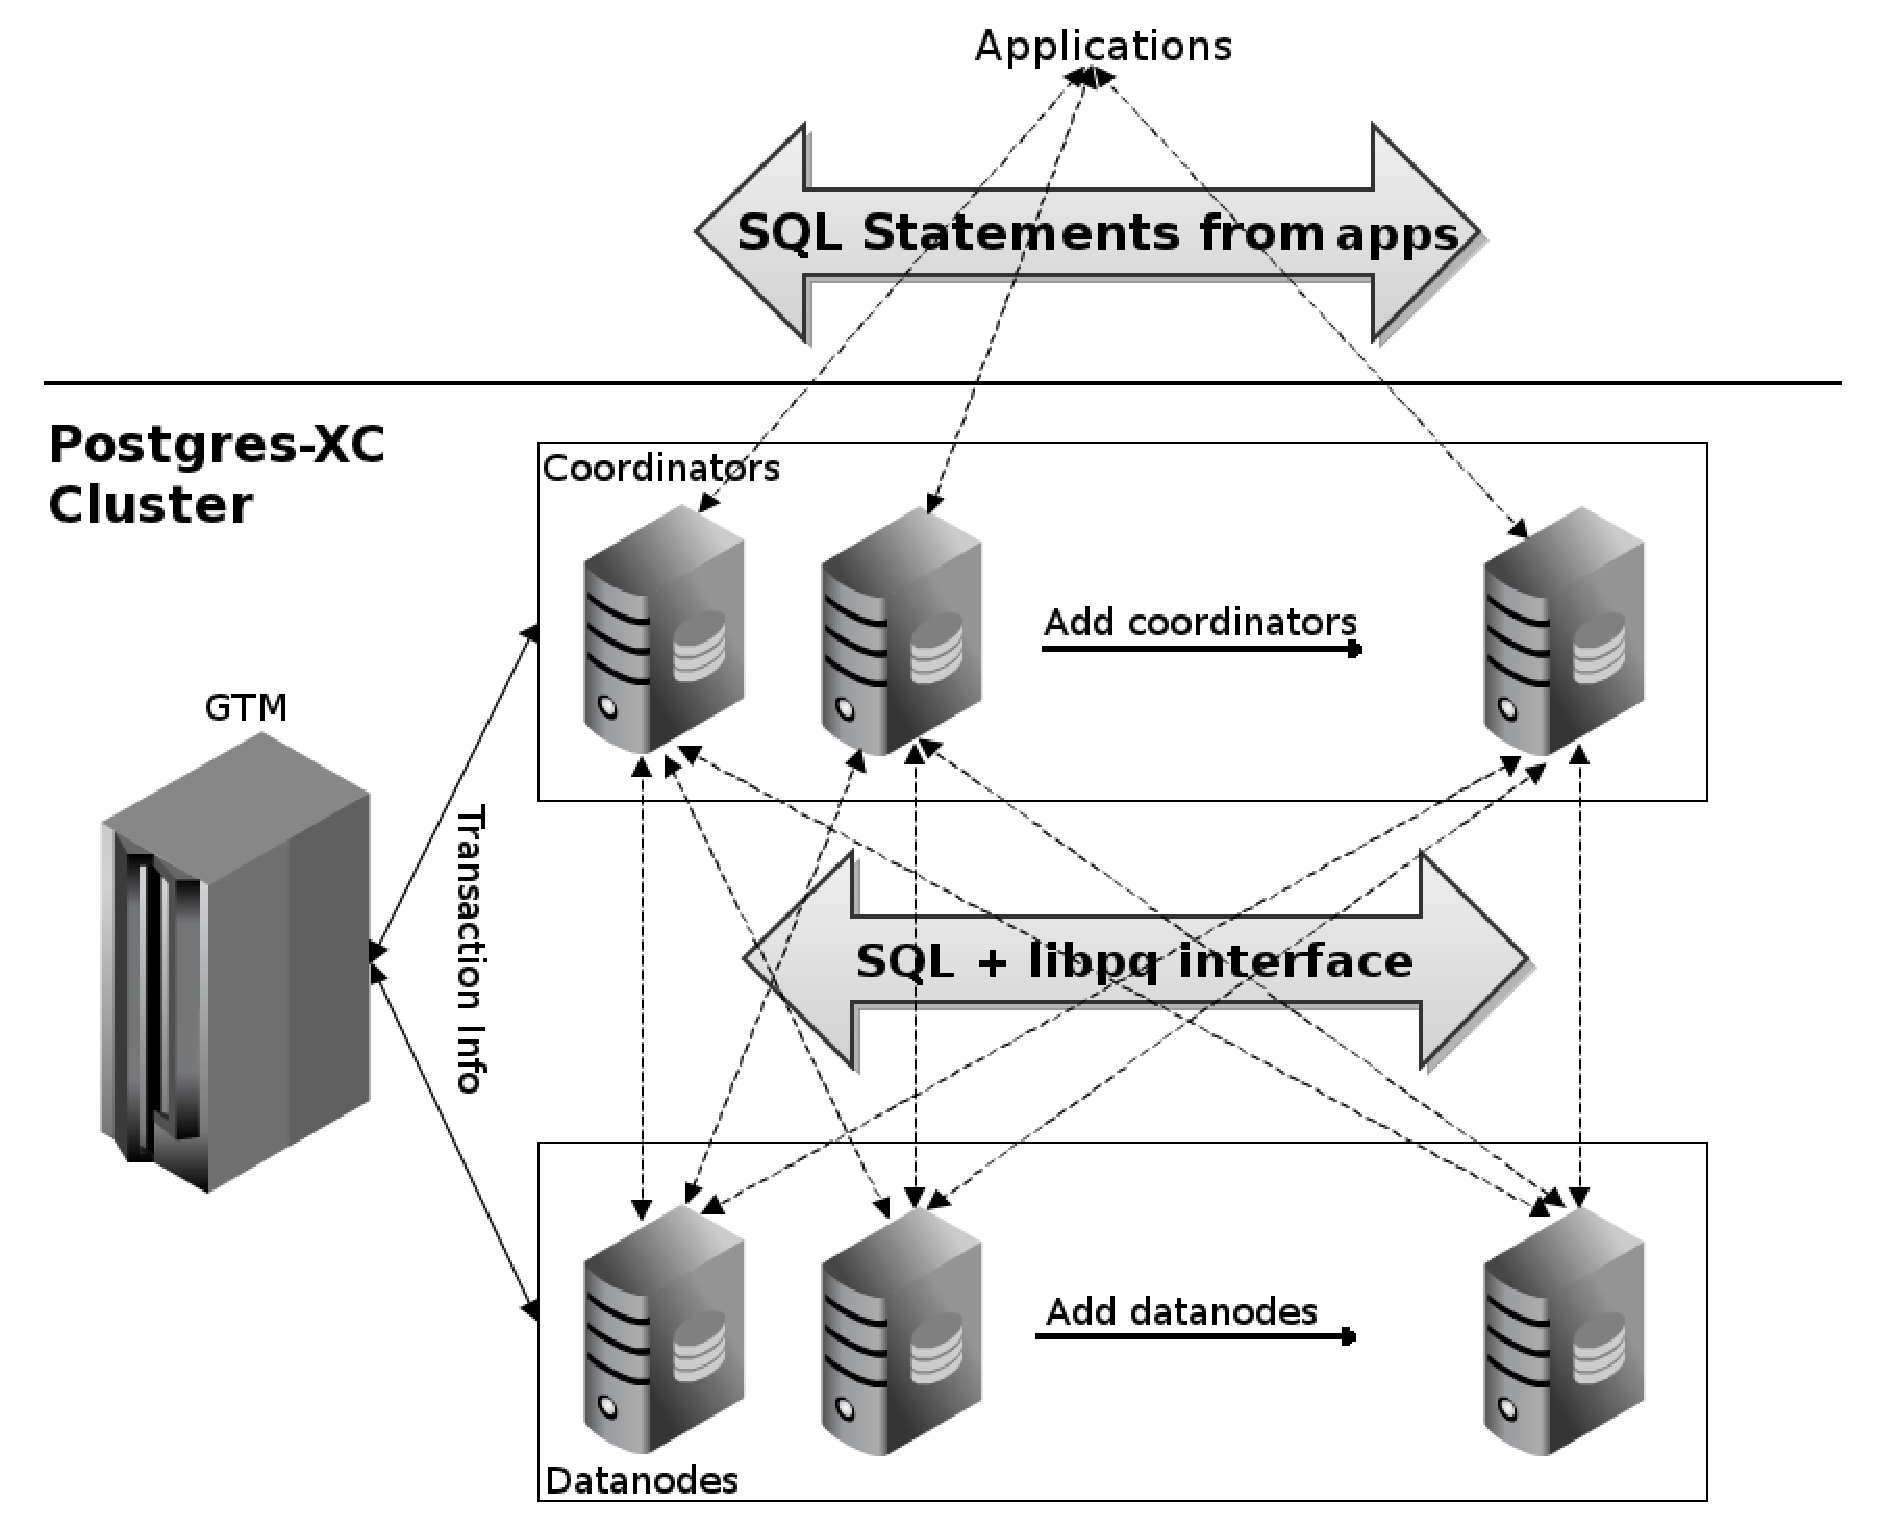
\includegraphics[width=1\textwidth]{postgres-xc-arch.pdf}}
  \caption{Архитектура Postgres-XC}
  \label{fig:postgres-xc1}
\end{figure}

Рис.~\ref{fig:postgres-xc1} показывает архитектуру Postgres-XC с тремя её основными компонентами:

\begin{enumerate}
\item Глобальный менеджер транзакций (GTM)~--- собирает и обрабатывает информацию о транзакциях в Postgres-XC, решает вопросы глобального идентификатора транзакции по операциям (для поддержания согласованного представления базы данных на всех узлах). Он обеспечивает поддержку других глобальных данных, таких как последовательности и временные метки. Он хранит данные пользователя, за исключением управляющей информации.
\item Координаторы (coordinators)~--- обеспечивают точку подключения для клиента (приложения). Они несут ответственность за разбор и выполнение запросов от клиентов и возвращение результатов (при необходимости). Они не хранят пользовательские данные, а собирать их из обработчиков данных (datanodes) с помощью запросов SQL через PostgreSQL интерфейс. Координаторы также обрабатывать данные, если требуется, и даже управляют двухфазной фиксацией. Координаторы используются также для разбора запросов, составления планов запросов, поиска данных и т.д.
\item Обработчик данных (datanodes)~--- обеспечивают сохранения пользовательских данных. Datanodes выполняют запросы от координаторов и возвращают им полученый результат.
\end{enumerate}

\subsection{Установка}

Установить Postgres-XC можно из \href{http://postgres-xc.sourceforge.net/docs/1_0/install-short.html}{исходников} или же из пакетов системы. Например в Ubuntu 12.10 можно установить postgres-xc так:

\begin{lstlisting}[label=lst:postgres-xc1,caption=Установка Postgres-XC]
sudo apt-get install postgres-xc postgres-xc-client postgres-xc-contrib postgres-xc-server-dev
\end{lstlisting}

По-умолчанию он создаст один координатор и два обработчика данных.

\subsection{Распределение данных и масштабируемость}

Postgres-XC предусматривает два способа хранения данных в таблицах:

\begin{figure}[ht!]
  \center{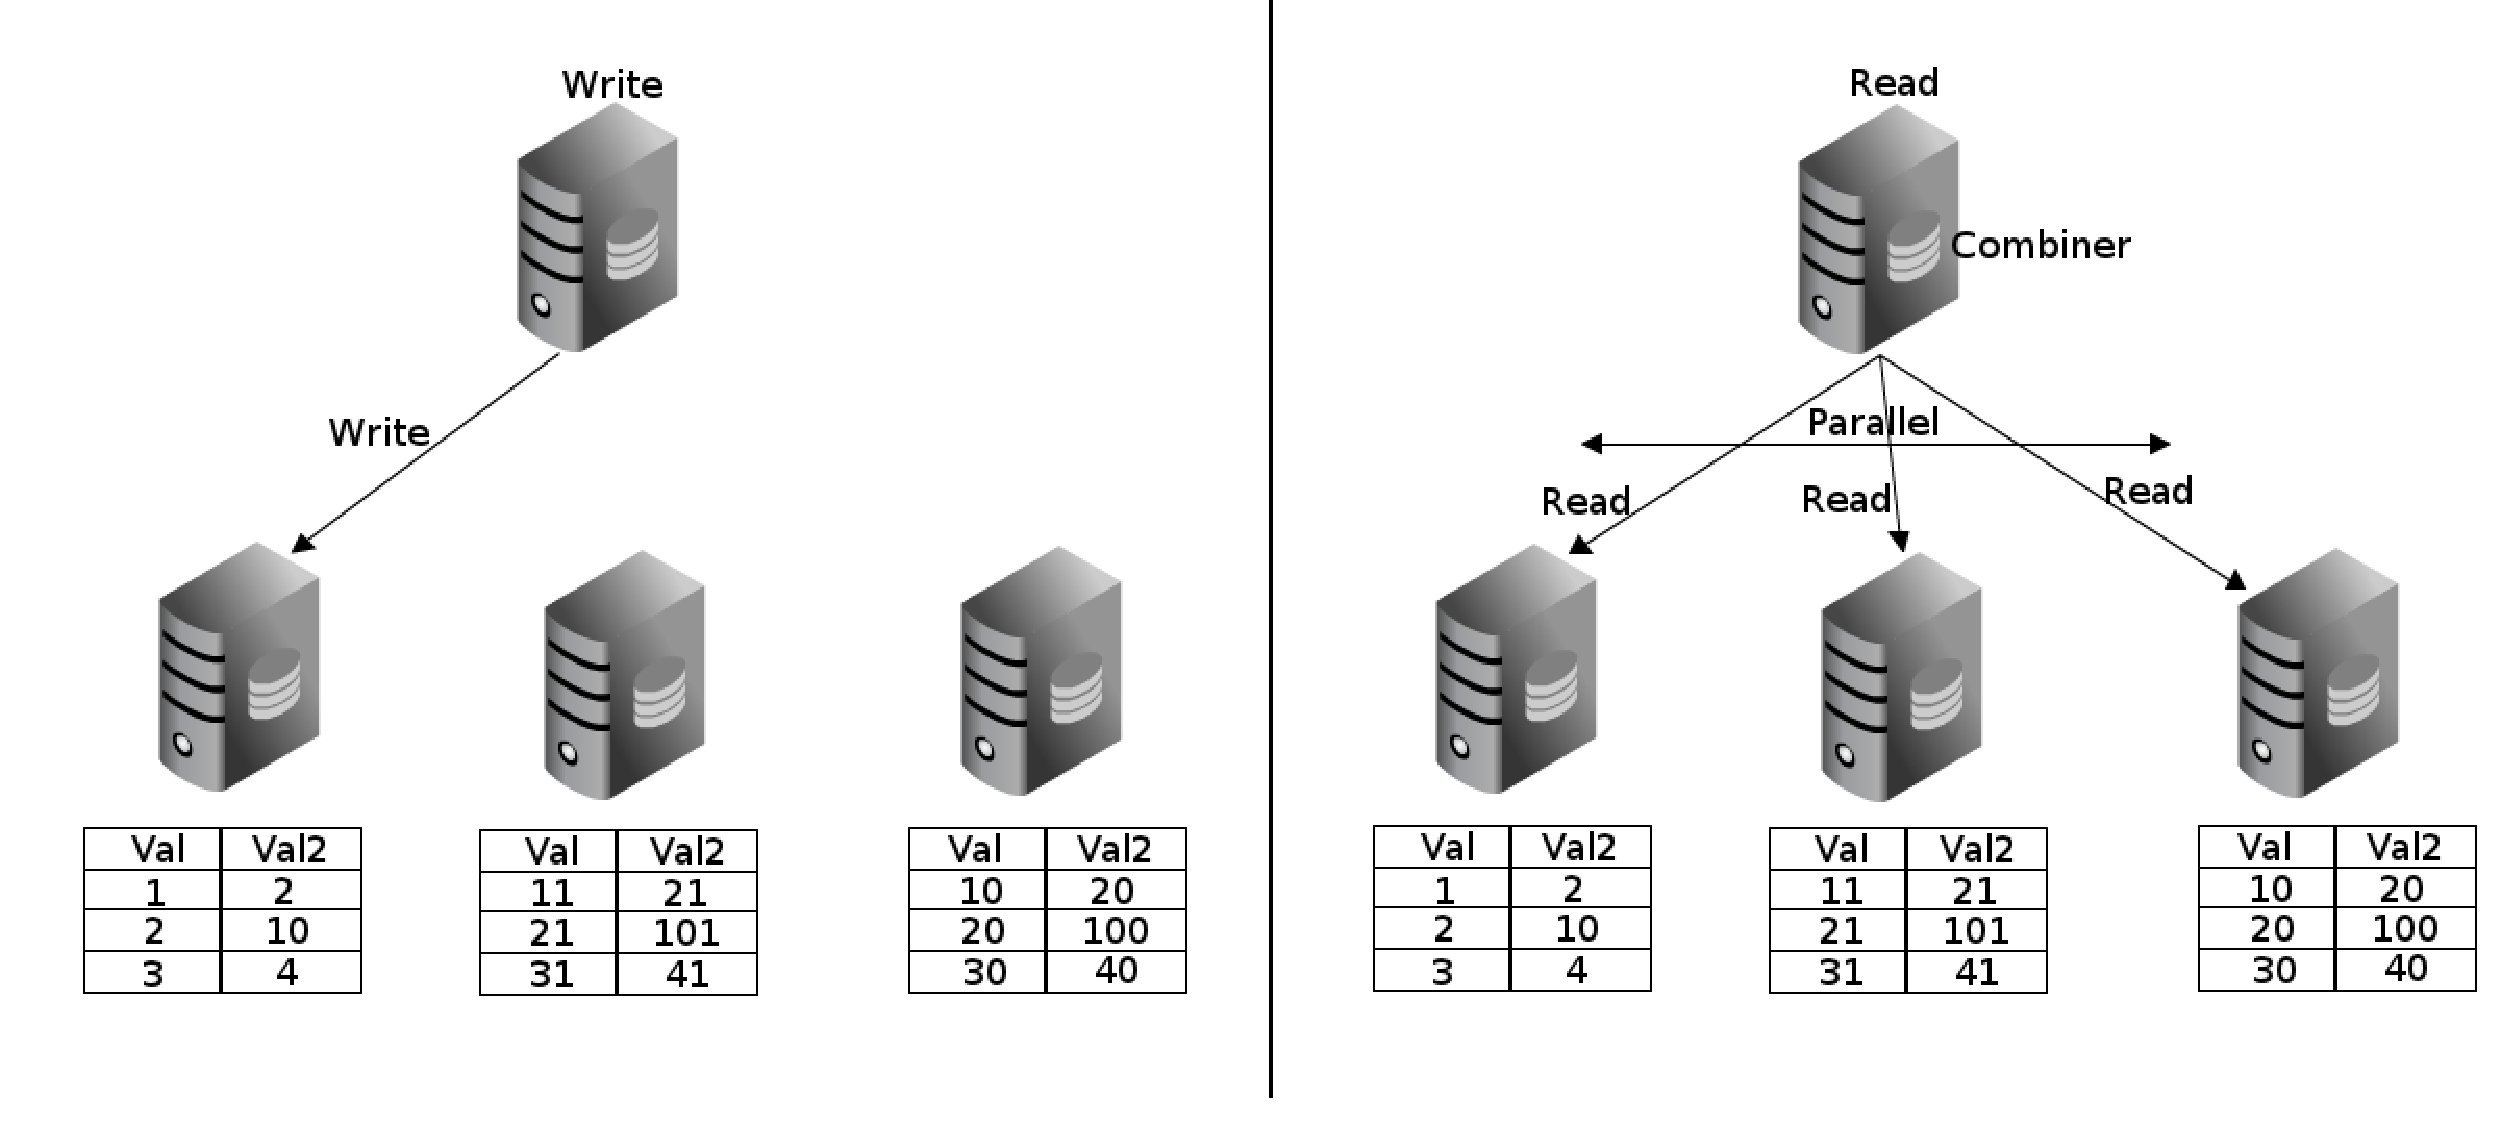
\includegraphics[width=1\textwidth]{postgres-xc-02.pdf}}
  \caption{Распределенные таблицы}
  \label{fig:postgres-xc2}
\end{figure}

\begin{figure}[ht!]
  \center{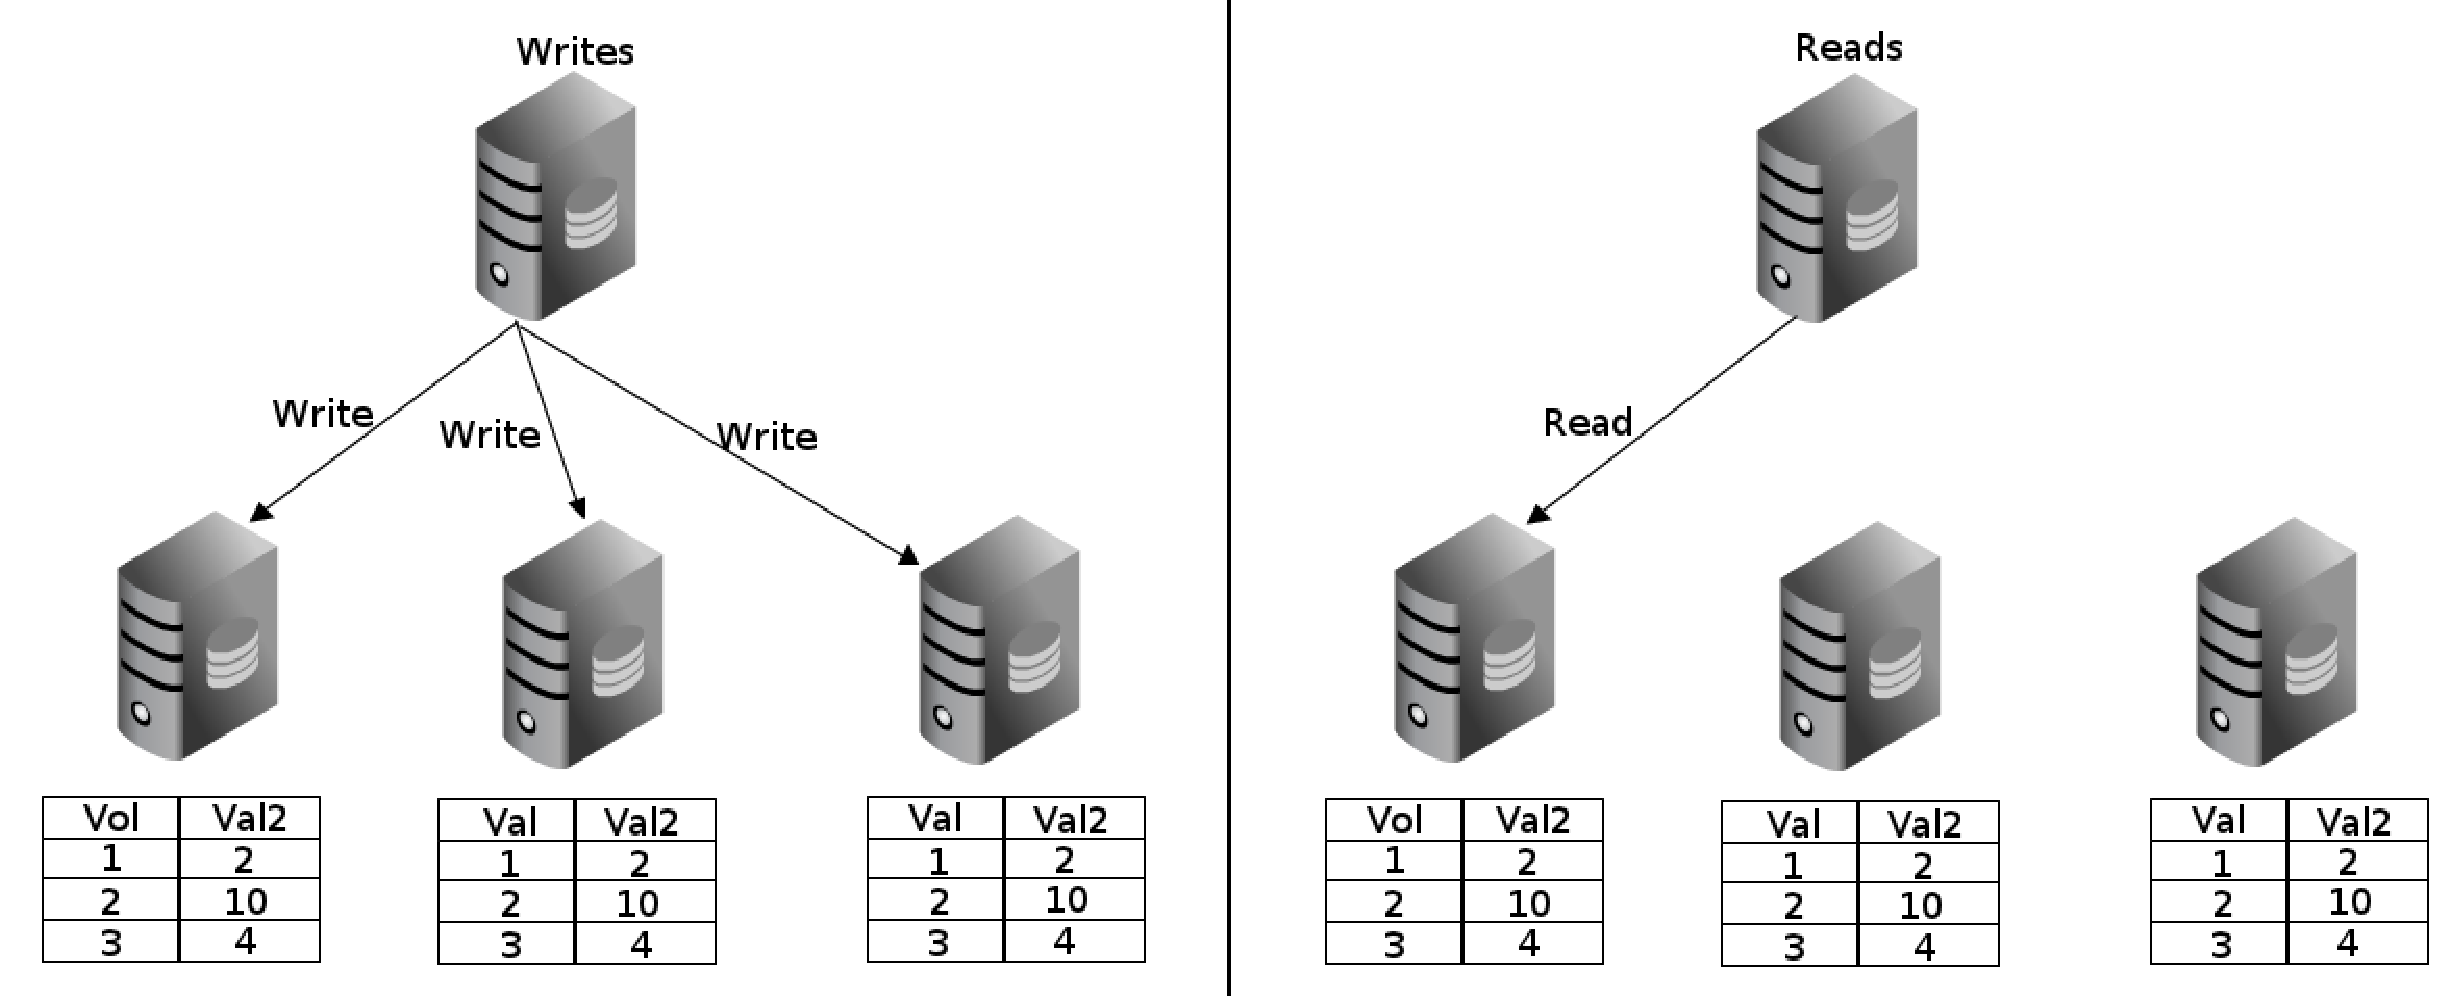
\includegraphics[width=1\textwidth]{postgres-xc-03.pdf}}
  \caption{Реплицированные таблицы}
  \label{fig:postgres-xc3}
\end{figure}

\begin{enumerate}
\item Распределенные таблицы (distributed tables, рис.~\ref{fig:postgres-xc2}): данные по таблице распределяются на указаный набор обработчиков данных с использованием указаной стратегии (hash, round-robin, modulo). Каждая запись в таблице находится только на одном обработчике данных. Паралельно могут быть записаны или прочитаны данные с различных обработчиков данных. За счет этого значительно улучшена производительность на запись и чтение.
\item Реплицированные таблицы (replicated tables, рис.~\ref{fig:postgres-xc3}): данные по таблице реплицируется (клонируются) на указаный набор обработчиков данных. Каждая запись в таблице находится на всех обработчиках данных (которые были указаны) и любые изменения дублируются на все обработчики данных. Так как все данные доступны на любом обработчике данных, координатор может собрать все данные из одного узла, что позволяет направить различные запросы на различные обработчики данных. Таким образом создается балансировка нагрузки и увеличения пропускной способности на чтение.
\end{enumerate}

\subsection{Высокая доступность (HA)}

По архитектуре у Postgres-XC всегда есть согласованность данных. По теореме CAP\footnote{http://en.wikipedia.org/wiki/CAP\_theorem} в такой системе тяжело обезпечить высокую доступность. Для достижения высокой доступности в распределенных системах требуется избыточность данных, резервные копии и автоматическое восстановление. В Postgres-XC избыточность данных может быть достигнута с помощью PostgreSQL потоковой (streaming) репликации с hot-standby для обработчиков данных. Каждый координатор способен записывать и читать данные независимо от другого, поэтому координаторы способны заменять друг друга. Поскольку GTM отдельный процесс и может стать точкой отказа, лучше создать GTM-standby как резервную копию. Ну а вот для автоматического восстановления придется использовать сторонние утилиты.

